% ---------------------------------------------------------------- 19
\begin{frame}{Le théorème de Bayes}
\begin{columns}[t]
\begin{column}{0.50\textwidth}
\begin{tcolorbox}[enhanced,colback=byDeep!6,colframe=byBlue,arc=2mm,
   boxrule=1pt,left=2mm,right=2mm,top=2mm,bottom=2mm]
\centering\large
\[
\underbrace{p(\theta \given y)}_{\text{a posteriori}}
\;=\;
\frac{\overbrace{p(y \given \theta)}^{\text{vraisemblance}}\;
      \overbrace{p(\theta)}^{\text{a priori}}}
     {\underbrace{\int p(y \given \theta')\,p(\theta')\,\mathrm{d}\theta'}_{\text{constante de normalisation}}}
\]
\end{tcolorbox}
\vspace{1mm}
\centering\small Forme proportionnelle, celle qu'on utilise en pratique :
\[\boxed{\;p(\theta \given y) \;\propto\; p(y \given \theta)\,p(\theta)\;}\]
\end{column}
\begin{column}{0.48\textwidth}
\begin{kbox}[Pourquoi c'est vrai]
Par définition de la probabilité conditionnelle :
\[
p(\theta \given y) = \frac{p(\theta, y)}{p(y)}
= \frac{p(y \given \theta)\,p(\theta)}{p(y)}
\]
et $p(y) = \int p(y \given \theta)p(\theta)\,\mathrm{d}\theta$
ne dépend \textbf{pas} de $\theta$.
\end{kbox}
\begin{wbox}[Le mot qui change tout]
L'intégrale du dénominateur est la \textbf{vraisemblance marginale}
$p(y)$ : c'est \emph{elle} qui décidera du facteur de Bayes et de la comparaison
de modèles (chapitre 4). Ici, on peut l'ignorer grâce à la proportionnalité.
\end{wbox}
\end{column}
\end{columns}
\end{frame}

% ---------------------------------------------------------------- 20
\begin{frame}{Démonstration pas à pas (3 lignes)}
\begin{abox}[On reprend la pièce truquée : prior Beta$(1,1)$, 7 faces sur 10]
\[
\begin{aligned}
\text{1. A priori}\quad & p(\theta) = \frac{\Gamma(2)}{\Gamma(1)\Gamma(1)}\theta^{0}(1-\theta)^{0} = 1 \\[1.5mm]
\text{2. Vraisemblance}\quad & p(y \given \theta) = \binom{10}{7}\theta^{7}(1-\theta)^{3} \\[1.5mm]
\text{3. Produit}\quad & p(\theta \given y) \propto \underbrace{\theta^{7}(1-\theta)^{3}}_{\text{le noyau seulement}}
\end{aligned}
\]
\end{abox}
\vspace{1mm}
\begin{solbox}[Reconnaître un noyau connu]
La forme $\theta^{7}(1-\theta)^{3}$ est le noyau d'une loi Beta de paramètres
$a-1 = 7$ et $b-1 = 3$, donc $a = 8$, $b = 4$ :
\[
p(\theta \given y) = \mathrm{Beta}(8,4) = \frac{\Gamma(12)}{\Gamma(8)\Gamma(4)}\theta^{7}(1-\theta)^{3}
\]
\textbf{La constante de normalisation n'a jamais eu besoin d'être calculée} : on l'a
retrouvée en reconnaissant le noyau. C'est le mécanisme de la conjugaison.
\end{solbox}
\end{frame}

% ---------------------------------------------------------------- 21
\begin{frame}{Bayes en quatre mots et en continu}
% [rogna]
\small
\begin{columns}[t]
\begin{column}{0.48\textwidth}
\begin{kbox}[Cas discret : la version de base]
\[
P(H \given E) = \frac{P(E \given H)\,P(H)}{P(E)}
\]
\begin{itemize}
  \item $H$ : hypothèse (malade, spam, modèle)
  \item $E$ : évidence (test positif, mot « gain »)
  \item $P(H)$ : croyance \emph{avant}
  \item $P(H \given E)$ : croyance \emph{après}
\end{itemize}
\end{kbox}
\begin{ebox}[Cotes, plus commode]
\[
\underbrace{\frac{P(H \given E)}{P(\bar H \given E)}}_{\text{cotes post.}}
=
\underbrace{\frac{P(H)}{P(\bar H)}}_{\text{cotes pri.}}
\times
\underbrace{\frac{P(E \given H)}{P(E \given \bar H)}}_{\text{rapport de vraisemblance}}
\]
Avec le spam : $0{,}25 \times 12 = 3 \Rightarrow P = 3/4 = 0{,}75$.
\end{ebox}
\end{column}
\begin{column}{0.48\textwidth}
\begin{ebox}[Cas continu : le paramètre]
\[
p(\theta \given y_1, \dots, y_n) \propto p(\theta)\prod_{i=1}^{n} p(y_i \given \theta)
\]
\begin{itemize}
  \item $\theta \in \R^d$ : paramètre (vecteur)
  \item $p(\theta)$ : densité a priori
  \item l'\textbf{i.i.d.} transforme le produit en somme de log
\end{itemize}
\end{ebox}
\begin{wbox}[Trois confusions classiques]
\begin{itemize}
  \item $p(\theta \given y) \neq p(y \given \theta)$ : les deux ne sont
        \textbf{pas} symétriques, la seconde est la vraisemblance.
  \item Une densité peut dépasser 1 : seule l'aire vaut 1.
  \item Le posterior \emph{dépend} du prior.
\end{itemize}
\end{wbox}
\end{column}
\end{columns}
\end{frame}

% ---------------------------------------------------------------- 22
\begin{frame}{Exercice guidé 1 --- détection de spam (10 min) --- l'énoncé}
\begin{ebox}[Énoncé]
Un filtre doit classer un courriel. On sait que :
\begin{itemize}
  \item 20 \% des courriels reçus sont des spams : $P(S) = 0{,}20$
  \item le mot « gain » apparaît dans 60 \% des spams : $P(G \given S) = 0{,}60$
  \item il apparaît dans 5 \% des courriels légitimes : $P(G \given \bar S) = 0{,}05$
\end{itemize}
\vspace{1.5mm}
\noindent\textbf{Question :} le mot « gain » est présent. Quelle est la probabilité
que ce courriel soit un spam ?
\end{ebox}
\vspace{1mm}
\begin{abox}[Question bonus (celle qui fait réfléchir)]
Et si « gain » apparaît \textbf{deux fois} ? \textbf{Quatre fois} ?
Quelle hypothèse êtes-vous obligé de faire ?
\end{abox}
\end{frame}

\begin{frame}{Exercice guidé 1 --- détection de spam}
\begin{center}
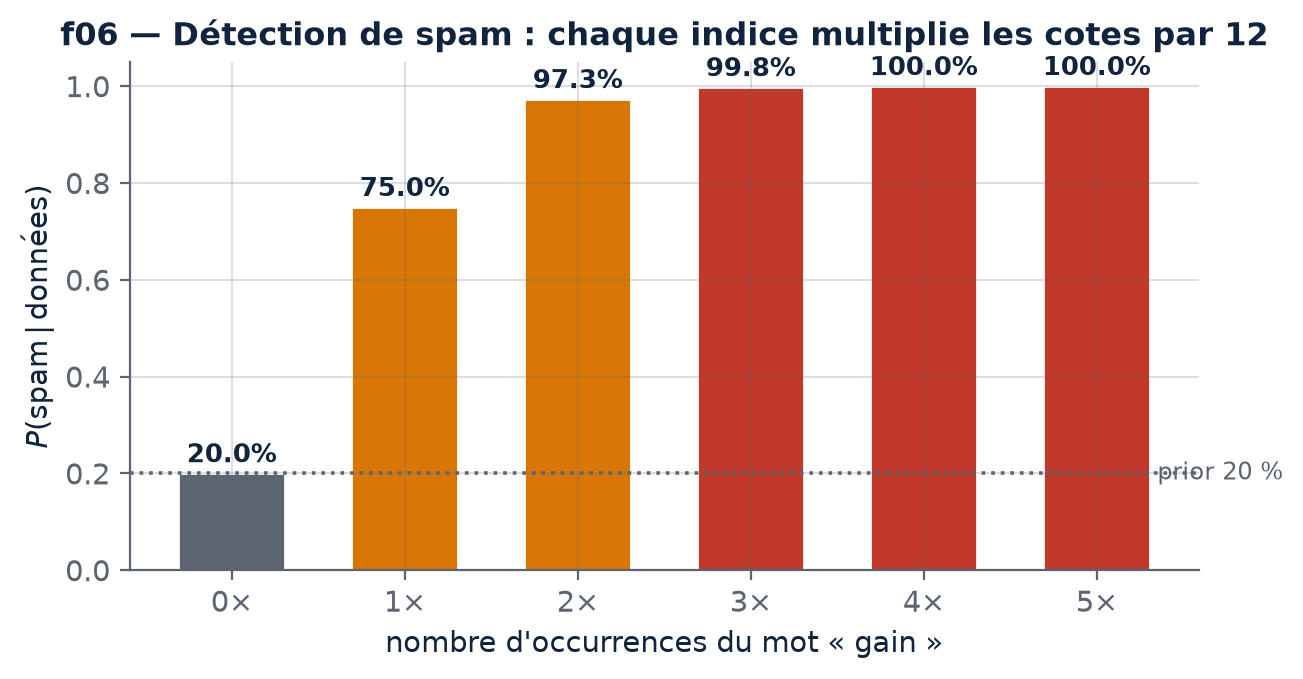
\includegraphics[width=.88\textwidth]{f06_spam.png}
\end{center}
\end{frame}

% ---------------------------------------------------------------- 23
\begin{frame}{Exercice guidé 1 — solution détaillée}
% [rogna]
\small
\begin{columns}[t]
\begin{column}{0.52\textwidth}
\begin{solbox}[Dénominateur d'abord]
\[
\begin{aligned}
P(G) &= P(G \given S)P(S) + P(G \given \bar S)P(\bar S)\\
     &= 0{,}60 \times 0{,}20 + 0{,}05 \times 0{,}80\\
     &= 0{,}12 + 0{,}04 = 0{,}16
\end{aligned}
\]
puis
\[
P(S \given G) = \frac{0{,}60 \times 0{,}20}{0{,}16} = 0{,}75
\]
Le score a été multiplié par 3 : les cotes passent de $1/4$ à $3/1$.
\end{solbox}
\end{column}
\begin{column}{0.46\textwidth}
\begin{ebox}[Occurrences répétées]
En supposant les occurrences \textbf{conditionnellement indépendantes} :
\[
P(S \given 2G) = \frac{0{,}60^2 \times 0{,}20}{0{,}60^2 \times 0{,}20 + 0{,}05^2 \times 0{,}80}
\]
\centering
\begin{tabular}{@{}lll@{}}
\toprule
Occurrences & Cotes & $P(S \given \cdot)$ \\
\midrule
0 & $0{,}25$ & 0,200 \\
1 & $3{,}0$ & \textbf{0,750} \\
2 & $36{,}0$ & \textbf{0,973} \\
3 & $432{,}0$ & \textbf{0,9977} \\
\bottomrule
\end{tabular}
\end{ebox}
\end{column}
\end{columns}
\vspace{1mm}
\begin{wbox}[Correction d'une erreur répandue]
On lit souvent « 2 occurrences $\Rightarrow$ 90 \% ». C'est faux : le calcul exact donne
\textbf{97,3 \%} ($0{,}25 \times 12^2 = 36$, soit $36/37$). Le facteur de Bayes se multiplie,
il ne s'additionne pas.
\end{wbox}
\end{frame}

% ---------------------------------------------------------------- 24
\begin{frame}{Quiz 2 — application directe}
\begin{qbox}[Question 2 -- Facteur 12]
Un filtre bayésien part d'un prior $P(S) = 0{,}20$ et traite chaque indice
indépendant comme un rapport de vraisemblance de 12.
\vspace{2mm}
Il faut dépasser 99 \% de certitude pour bloquer sans revue humaine.
Combien d'indices faut-il au minimum ?
\vspace{2mm}
\begin{enumerate}
  \item[(A)] 2 \quad \item[(B)] 3 \quad \item[(C)] 4 \quad \item[(D)] 6
\end{enumerate}
\vspace{2mm}
\textbf{Réponse : (B)} --- les cotes valent $0{,}25 \times 12^k$ ;
$k = 3$ donne 432, soit $0{,}9977 > 0{,}99$. Avec $k = 2$ on plafonne à 0,973.
\end{qbox}
\vspace{1.5mm}
\begin{kbox}[Ce que ce petit calcul enseigne]
La \textbf{mise à jour séquentielle} est une addition de log-cotes :
$\log(\text{cotes post.}) = \log(\text{cotes pri.}) + \sum_k \log(\text{LR}_k)$.
C'est exactement l'architecture d'un Naive Bayes, et c'est la raison pour laquelle
il tient sur un téléphone.
\end{kbox}
\end{frame}

% ---------------------------------------------------------------- 25
\begin{frame}{Exercice guidé 2 — le test COVID (10 min)}
\begin{columns}[t]
\begin{column}{0.47\textwidth}
\begin{ebox}[Énoncé]
Un test antigénique a
\begin{itemize}
  \item sensibilité $P(T^+ \given M) = 0{,}95$
  \item spécificité $P(T^- \given \bar M) = 0{,}98$
\end{itemize}
On teste une personne tirée au hasard dans une population où la prévalence est
de \textbf{5 \%}.
\vspace{1.5mm}
\textbf{Question :} le test est positif.
Quelle est la probabilité qu'elle soit réellement malade ?
\vspace{1.5mm}

\noindent\textcolor{byBlue}{\textbf{Indice :}} commencez par compter sur 1000 personnes.
\end{ebox}
\end{column}
\begin{column}{0.51\textwidth}
\begin{solbox}[Résolution en arbre]
Sur 1000 personnes :
\begin{itemize}
  \item 50 malades : $50 \times 0{,}95 = 47{,}5$ positifs
  \item 950 saines : $950 \times 0{,}02 = 19$ faux positifs
\end{itemize}
\[
P(M \given T^+) = \frac{47{,}5}{47{,}5 + 19} = \frac{47{,}5}{66{,}5} = \mathbf{0{,}714}
\]
\centering\footnotesize
Même sensibilité, même spécificité : la réponse dépend entièrement du contexte.
\end{solbox}
\end{column}
\end{columns}
\end{frame}

% ---------------------------------------------------------------- 26
% [split]
\begin{frame}{Le même test, six vérités différentes}
\begin{center}
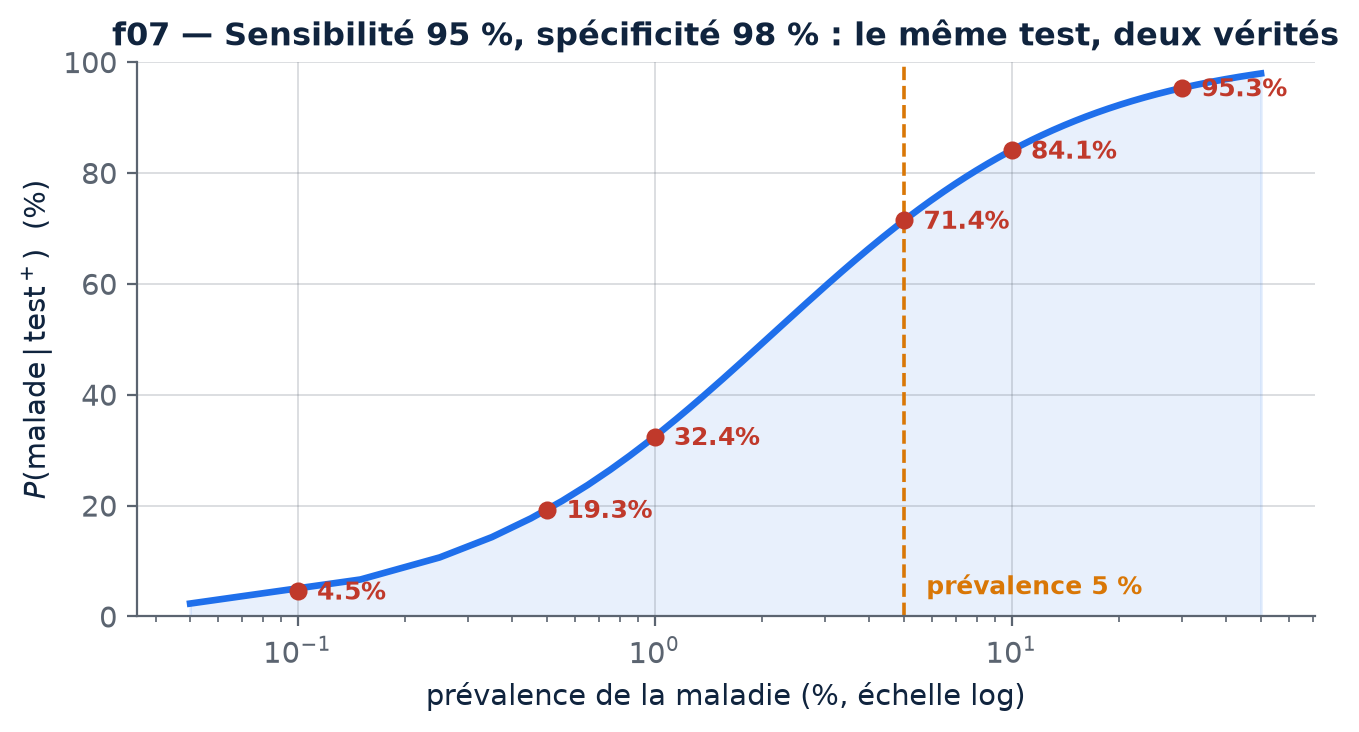
\includegraphics[width=.86\textwidth]{f07_covid_ppv.png}
\end{center}
\end{frame}

% [split]
\begin{frame}{Le même test, six vérités différentes}

\vspace{-1mm}
\begin{columns}[t]
\begin{column}{0.62\textwidth}
\begin{tabular}{@{}lcccccc@{}}
\toprule
Prévalence & 0,1 \% & 0,5 \% & 1 \% & 5 \% & 10 \% & 30 \% \\
\midrule
$P(M \given T^+)$ & 4,5 \% & 19,3 \% & 32,4 \% & \textbf{71,4 \%} & 84,1 \% & 95,3 \% \\
\bottomrule
\end{tabular}
\vspace{1.5mm}

\small Toutes ces valeurs sortent du calcul exécuté dans \file{src/fig\_ch1.py}.
\end{column}
\begin{column}{0.36\textwidth}
\begin{kbox}[Le cœur du cours]
La prévalence \textbf{est} un prior. La formule de Bayes n'est pas une recette de
calcul : c'est la déclaration explicite qu'\emph{une conclusion dépend de ce qu'on
croyait avant de mesurer}.
\end{kbox}
\end{column}
\end{columns}
\end{frame}
